% ----------------------------------------------------------------- %
%             The Speech Signal Processing Toolkit (SPTK)           %
%             developed by SPTK Working Group                       %
%             http://sp-tk.sourceforge.net/                         %
% ----------------------------------------------------------------- %
%                                                                   %
%  Copyright (c) 1984-2007  Tokyo Institute of Technology           %
%                           Interdisciplinary Graduate School of    %
%                           Science and Engineering                 %
%                                                                   %
%                1996-2017  Nagoya Institute of Technology          %
%                           Department of Computer Science          %
%                                                                   %
% All rights reserved.                                              %
%                                                                   %
% Redistribution and use in source and binary forms, with or        %
% without modification, are permitted provided that the following   %
% conditions are met:                                               %
%                                                                   %
% - Redistributions of source code must retain the above copyright  %
%   notice, this list of conditions and the following disclaimer.   %
% - Redistributions in binary form must reproduce the above         %
%   copyright notice, this list of conditions and the following     %
%   disclaimer in the documentation and/or other materials provided %
%   with the distribution.                                          %
% - Neither the name of the SPTK working group nor the names of its %
%   contributors may be used to endorse or promote products derived %
%   from this software without specific prior written permission.   %
%                                                                   %
% THIS SOFTWARE IS PROVIDED BY THE COPYRIGHT HOLDERS AND            %
% CONTRIBUTORS "AS IS" AND ANY EXPRESS OR IMPLIED WARRANTIES,       %
% INCLUDING, BUT NOT LIMITED TO, THE IMPLIED WARRANTIES OF          %
% MERCHANTABILITY AND FITNESS FOR A PARTICULAR PURPOSE ARE          %
% DISCLAIMED. IN NO EVENT SHALL THE COPYRIGHT OWNER OR CONTRIBUTORS %
% BE LIABLE FOR ANY DIRECT, INDIRECT, INCIDENTAL, SPECIAL,          %
% EXEMPLARY, OR CONSEQUENTIAL DAMAGES (INCLUDING, BUT NOT LIMITED   %
% TO, PROCUREMENT OF SUBSTITUTE GOODS OR SERVICES; LOSS OF USE,     %
% DATA, OR PROFITS; OR BUSINESS INTERRUPTION) HOWEVER CAUSED AND ON %
% ANY THEORY OF LIABILITY, WHETHER IN CONTRACT, STRICT LIABILITY,   %
% OR TORT (INCLUDING NEGLIGENCE OR OTHERWISE) ARISING IN ANY WAY    %
% OUT OF THE USE OF THIS SOFTWARE, EVEN IF ADVISED OF THE           %
% POSSIBILITY OF SUCH DAMAGE.                                       %
% ----------------------------------------------------------------- %
\hypertarget{fig}{}
\name{fig}{plot a graph}{plotting graphs}

\begin{synopsis}
 \item[fig] [ --F $F$ ] [ --R $R$ ] [ --W $W$ ] [ --H $H$] [ --o $xo$ $yo$ ]
            [ --g $G$ ]  [ --p $P$ ] [ --j $J$ ]
 \item[\ ~~~] [ --s $S$ ] [ --f $file$ ] [ --t ] [ {\em infile} ]
\end{synopsis}

\begin{qsection}{DESCRIPTION}
{\em fig} draws a graph using information 
from {\em infile} (or standard input), 
sending the result in FP5301 plot format to standard output. 
This command is similar to the Unix command ``graph'' 
but includes some labeling functions. 
The output can be printed directly on a printer 
that supports the FP5301 protocol, 
displayed on an X11 display with the \hyperlink{xgr}{xgr} command, 
or converted to PostScript format with the \hyperlink{psgr}{psgr} command.
\end{qsection}

\begin{options}
        \argm{F}{F}{factor}{1}
        \argm{R}{R}{rotation angle}{0}
        \argm{W}{W}{width of figure ($\times 100$mm)}{1}
        \argm{H}{H}{height of figure ($\times 100$mm)}{1}
        \argm{o}{xo \; yo}{origin in mm}{20 20}
        \argm{g}{G}{draw grid ($0 \sim 2$)\\
                        \begin{tabular}{cccc}
                        &
\includegraphics[width=2cm]{fig/g0.pdf}
                        &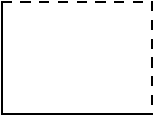
\includegraphics[width=2cm]{fig/g1.pdf}
                        &
\includegraphics[width=2cm]{fig/g2.pdf}\\
                        $G$&0&1&2        
                        \end{tabular}\\\hspace*{\fill}}{2}
        \argm{p}{P}{pen number ($1 \sim 10$)}{1}
        \argm{j}{J}{join number ($0 \sim 2$)}{0}
        \argm{s}{S}{font size ($1 \sim 4$)}{1}
        \argm{f}{file}{The file assigned after this option is read
                       before {\em infile}, that is, this option gives
                       preference.}{NULL}
        \argm{t}{}{transpose $x$ and $y$ axes}{FALSE}
\end{options}

\begin{qsection}{EXAMPLE}
In the example below, data in {\em data.fig} file is plotted in an X terminal:
\vspace{-3mm}
\begin{quote}
 \verb!fig data.fig |xgr!
\end{quote}
\vspace{-3mm}
In this example, data in {\em data.fig} file is converted to postscript format
and visualized with ghostview:
\vspace{-3mm}
\begin{quote}
 \verb!fig data.fig | psgr | ghostview -!
\end{quote}
\vspace{-3mm}
\end{qsection}

\vspace{-1cm}
\begin{qsection}{USAGE}
~\vspace{-1cm}
\end{qsection}

\begin{qsection}{\ ~~~COMMAND}
The input data file can contain commands and data.
Commands can be used for labeling, scaling, etc.
Data is written in the ($x ~y$) coordinate pair form.
Command values can be overwritten by entering new command values.
\end{qsection}

\vspace{-1cm}
\begin{qsection}{\ ~~~COMMAND LINES}
\begin{minipage}[t]{5.5cm}
x [mel $\alpha$]~ $xmin$ ~$xmax$ [$xa$]\\
y [mel $\alpha$]~ $ymin$ ~$ymax$ [$ya$]\\
\end{minipage}
\begin{minipage}[t]{9cm}
Assigns $x$ and $y$ scalings.
Marks can be specified in $x$ and $y$ axes through $xa$ and $ya$.
If no setting of $xa$ and $ya$ is done,
then $xa$ is set to $xmin$ and $ya$ to $ymin$.
If the optional ``mel $\alpha$'', where $\alpha$ must be
a number (for example, mel 0.35), is used,
then labeling is undertaken as a frequency transformation of
a minimum phase first order all-pass filter.
\end{minipage} \\

\begin{minipage}[t]{5.5cm}
xscale ~$x_1$ $x_2$ $x_3$ $\dots$\\
yscale ~$y_1$ $y_2$ $y_3$ $\dots$
\end{minipage}
\begin{minipage}[t]{9cm}
Assigns values to the points $x_1, x_2,x_3,\dots$
and $y_1,y_2,y_3,\dots$ in $x$ and $y$ axes.
These points can be assigned with numbers or marks,
Also, when one wants to specify points which consist of numeric and non-numeric
characters all together (like in '2,*.3.14), then the following function should
be used:
\begin{tabular}{cl}
s & draws marks with half size.\\
$\backslash$& only writes number.\\
@ & does not write anything \\
  & but assigns positions of marks.\\
none of the above & only marks are written.
\end{tabular}\\

Whenever the character is inside quotes,
it appears in the position assigned
by the string that precedes it.
Please refer to the commands \hyperlink{xyname}{x/yname} for information on
special characters.\\
(Example)\\
x ~0 ~5\\
xscale 0~1.0 ~s1.5 ~'2 ~$\backslash$2.5 ~'3.14 ~''$\backslash$pi'' ~@4 ~''x'' ~5\\

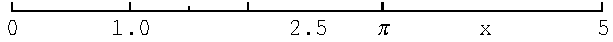
\includegraphics[width=9cm]{fig/scale.pdf}
\end{minipage}\\

\hypertarget{xyname}{}
\begin{minipage}[t]{5.5cm}
xname ~''$text$''\\
yname ~''$text$''\\
\end{minipage}
\begin{minipage}[t]{9cm}
Labels $x$ and $y$ axes.
$text$ should appear between the quotes.
Within $text$, \TeX commands can be used.
Also, characters, such as those that can be obtained
with \TeX, can be written with this command.
\end{minipage}\\

\begin{minipage}[t]{5.5cm}
 print ~x ~y ~''$text$'' [$th$]\\
 printc ~x ~y ~''$text$'' [$th$]
\end{minipage}
\begin{minipage}[t]{9cm}
This command writes $text$ in the position (x ~y) assigned.
The option $th$ sets the rotation degree.

\begin{tabular}{cc}
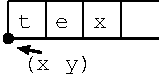
\includegraphics{fig/fig-print1.pdf}&  
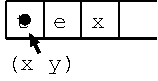
\includegraphics{fig/fig-print2.pdf}\\
print&printc
\end{tabular}p
\end{minipage}\\

\begin{minipage}[t]{5.5cm}
title ~x ~y ~''$text$'' [$th$]\\
titlec ~x ~y ~''$text$'' [$th$]
\end{minipage}
\begin{minipage}[t]{9cm}
This command does the same as print(c).
However, the basic unit is expressed in the mm, evaluated as absolute value.
The reference point is on the bottom-left side.
\end{minipage}\\

\begin{minipage}[t]{5.5cm}
csize ~h [w]
\end{minipage}
\begin{minipage}[t]{9cm}
This command sets the character width and height (in mm),
to be used in the following commands:\\
x/yscale, x/yname, print/c, title/c\\
When the value of $w$ is omitted, $w$ is made equal to $h$.
The default values for the option --{\bf s} are as follows:
\begin{tabular}{ccc}

--{\bf s} &w &h  \\ \hline
1 &2.5 &2.2\\
2&5&2.6\\
3&2.5&4.4\\
4&5&4.4
\end{tabular}\\

\end{minipage}\\

\begin{minipage}[t]{5.5cm}
 pen ~$penno$
\end{minipage}
\begin{minipage}[t]{9cm}
This command chooses the variable $penno$.
$1 \leq  penno \leq 10$
Please refer to \hyperlink{pen-color}{appendix}.
\end{minipage}\\

\begin{minipage}[t]{5.5cm}
 join ~$joinno$
\end{minipage}
\begin{minipage}[t]{9cm}
This command chooses the variable $joinno$.
$0 \leq joinno \leq 2$
Please refer to the \hyperlink{join-type}{appendix}.
\end{minipage}\\

\begin{minipage}[t]{5.5cm}
line ~$ltype$ [$lpt$]
\end{minipage}
\begin{minipage}[t]{9cm}
This command sets the type $ltype$ of the line which will connect
data as well as the $lpt$ pace. $lpt$ is in mm.
When $ltype$=0: no line is used to connect coordinate points.
1:~solid~~2:~dotted~~3:~dot and dash~~4:~broken~~5:~dash
Please refer to the \hyperlink{pen-line}{appendix}.\\
        
\end{minipage}\\

\begin{minipage}[t]{5.5cm}
xgrid ~$x_1$ ~$x_2$ ~$\dots$\\
ygrid ~$y_1$ ~$y_2$ ~$\dots$
\end{minipage}
\begin{minipage}[t]{9cm}
This command causes grids to be drawn in the positions $x_1$ $x_2$ $\dots$,
$y_1$ $y_2$ $\dots$.\\
(Example)\\
\begin{minipage}[t]{4.3cm}
 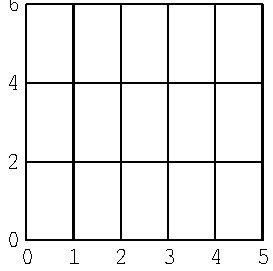
\includegraphics[width=4cm]{fig/grid.pdf}
\end{minipage}
\begin{minipage}[b]{4.5cm}
\baselineskip 5pt
x 0 5\\
y 0 6\\
xscale 0 1 2 3 4 5\\
yscale 0 2 4 6

\vspace{3mm}
xgrid 1 2 3 4\\
ygrid 2 4
\vspace*{1cm}
\end{minipage}
\end{minipage}\\


\begin{minipage}[t]{5.5cm}
mark ~$label$ [$th$]
\end{minipage}
\begin{minipage}[t]{9cm}
This command draws a mark in the assigned coordinate position.
The option $th$ specifies the angle(degree) in which the string will be draw.
If $label$ is assigned with $\backslash 0$, the mark is released.
A detailed explanation on writing marks and special characters to graphs is
 provided at the label section.
\end{minipage}\\

\begin{minipage}[t]{5.5cm}
height ~$h$ [$w$]\\
italic ~$th$
\end{minipage}
\begin{minipage}[t]{9cm}
The height command defines the size of the label through its
height $h$(mm) and width $w$(mm).
The labels may also be written in italic by using the italic command.
\end{minipage}\\

\begin{minipage}[t]{5.5cm}
circle ~x ~y ~$r_1$ ~$r_2$ ~$\dots$\\
xcircle ~x ~y ~$r_1$ ~$r_2$ ~$\dots$\\
ycircle ~x ~y ~$r_1$ ~$r_2$ ~$\dots$

\end{minipage}
\begin{minipage}[t]{9cm}
These commands write circles with radius $r_1$ ~$r_2$ ~$\dots$
and center on the coordinate ($x$,~$y$).
Also, the radius $r_x$ is given in mm.
As for the xcircle and ycircle commands,
the units considered for the radius are the scales of the $x$ axis and
 $y$ axis, respectively, as shown in the figure below.

(Example)\\
\begin{minipage}[t]{4.3cm}
 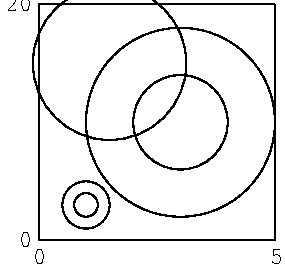
\includegraphics[width=4cm]{fig/circle.pdf}
\end{minipage}
\begin{minipage}[b]{4.5cm}
\baselineskip 5pt
x 0 5\\
y 0 20\\
xscale 0 5\\
yscale 0 20

\vspace*{3mm}
xcircle 3 10 1 2\\
ycircle 1 3 1 2\\
circle  1.5 15 13\\
\vspace*{7mm}
\end{minipage}
\end{minipage}\\

\begin{minipage}[t]{5.5cm}
box ~$x_0$ $y_0$ $x_1$ ~$y_1$ [~$x_2$ $y_2$ $\dots$ ]\\
paint ~$type$
\end{minipage}
\begin{minipage}[t]{9cm}
This command draws a rectangle with paint $type$
connecting ($x_0$ $y_0$) and ($x_1$ $y_1$) through a solid line.
The line which connects ($x_0$ $y_0$) and ($x_1$ $y_1$) forms
the diagonal of the rectangle.
Also, if $x_2$ $y_2$ $\dots$ are assigned, a polygon is draw connecting
the points ($x_0$ $y_0$),($x_1$ $y_1$),($x_2$ $y_2$),$\dots$.
In this case, Please do not set the paint $type$
 to any value different from the default.
The default value is 1.\\

(Example)\\
\begin{minipage}[t]{4.3cm}
 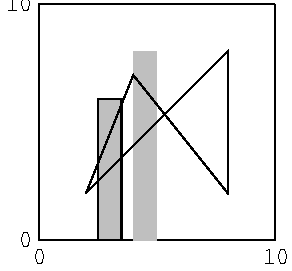
\includegraphics[width=4cm]{fig/box.pdf}
\end{minipage}
\begin{minipage}[b]{4.5cm}
\baselineskip 5pt
x 0 10\\
y 0 10\\
xscale 0 10\\
yscale 0 10

\vspace*{3mm}
paint 18\\
box 2.5 0 3.5 6\\
paint -18 \\
box 4 0 5 8\\
paint 1\\
box  2 2 8 8 8 2 4 7
\end{minipage}
\end{minipage}\\

\begin{minipage}[t]{5.5cm}
clip ~$x_0$ $y_0$ $x_1$ ~$y_1$ 
\end{minipage}
\begin{minipage}[t]{9cm}
This command allows for drawing only inside the box defined by
($x_0$ $y_0$), ($x_1$ $y_1$).
When the coordinates ($x_0$ $y_0$), ($x_1$ $y_1$) are omitted,
then the clip command is skipped.\\

(Example)\\
\begin{minipage}[t]{4.3cm}
 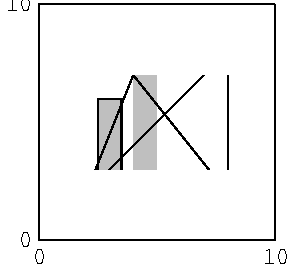
\includegraphics[width=4cm]{fig/clip.pdf}
\end{minipage}
\begin{minipage}[b]{4.5cm}
\baselineskip 5pt
x 0 10\\
y 0 10\\
xscale 0 10\\
yscale 0 10

\vspace*{3mm}
clip 2 3 9 7\\
paint 18\\
box 2.5 0 3.5 6\\
paint -18 \\
box 4 0 5 8\\
paint 1\\
box  2 2 8 8 8 2 4 7
\end{minipage}
\end{minipage}\\

\begin{minipage}[t]{5.5cm}
\# any comment
\end{minipage}
\begin{minipage}[t]{9cm}
This is used for writing comment lines.
Whatever is written after the symbol $\#$
is ignored by the fig command.
\end{minipage}\\
\end{qsection}

\begin{qsection}{\ ~~~DATA LINES}
\begin{minipage}[t]{5.5cm}
 x ~y [$label$~ [$th$]]
\end{minipage}
\begin{minipage}[t]{9cm}
The coordinates (x ~y) are scaled by the values specified in the
command line.
If a string is written to $label$, then it will be written
in the (x ~y) position.
There should be no empty characters (e.g., space) in the beginning of the label
setting.
When $label$ is given in the mark command,
the $label$ replacement will take place only for this coordinate.
The option $th$ assigns the angle.\\
If $\backslash n$, where $0 \leq n \leq 15$, is assigned to $label$,
the corresponding mark is draw (refer to the \hyperlink{lmark}{appendix} for the types of
marks).
When a minus sign is written before mark number,
then the connecting line between marks passes through the center of
each mark.\\
If a minus sign is not included, then connecting lines do not pass
through the center of each mark.
When $n=16(\backslash 16)$, a small circle is written with
diameter defined by the hight command.
Also, special character and ASCII character can be written through
code number when $n>32$.
\end{minipage}\\

\begin{minipage}[t]{5.5cm}
 eod\\
EOD
\end{minipage}
\begin{minipage}[t]{9cm}
This is the end of data sign.
Coordinates before and after the eod sign are not connected.
\end{minipage}
\end{qsection}
\newpage
\begin{qsection}{APPENDIX}
\hypertarget{lmark}{}
{\large \hspace{-1.5ex}$\bullet$
The following type of marks can be defined through $label$:}

\begin{center}
\leavevmode
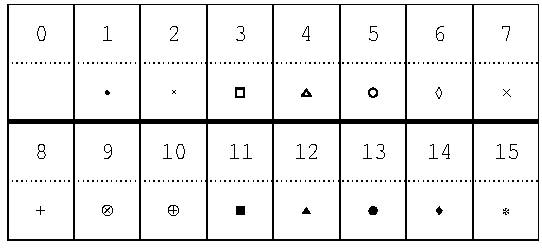
\includegraphics[width=12cm]{fig/mark.pdf} \\
\end{center}

\hypertarget{pen-line}{}
{\large \hspace{-1.5ex}$\bullet$
The following types of pen and line can be defined:}\\
\hspace{3mm}[When output is obtained through the command \hyperlink{psgr}{psgr}]

\leavevmode
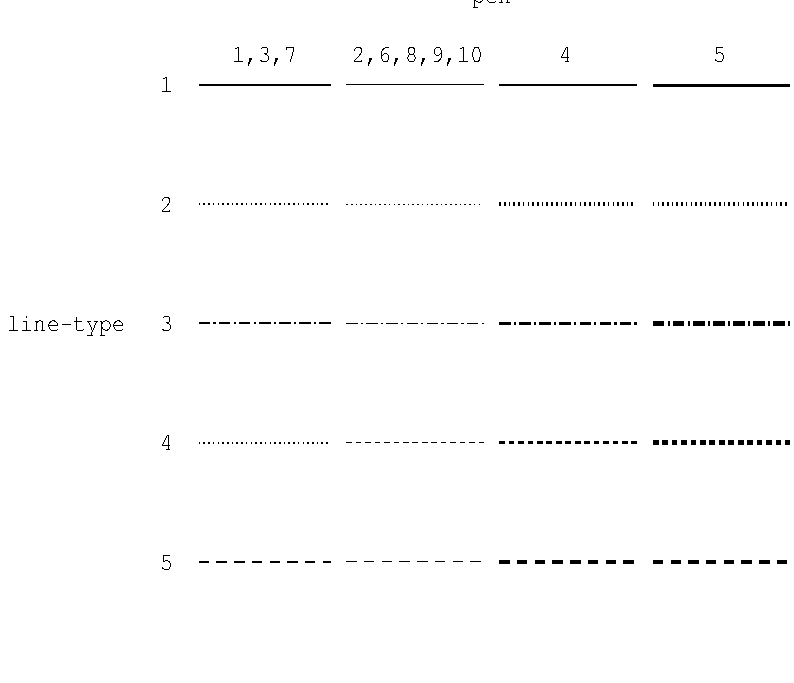
\includegraphics{fig/pen-line.pdf} \\

ps:~~ The types of output generated by the pen command
depend on the printer (Please try printing this page).
\newpage
[When output is obtained through the command \hyperlink{xgr}{xgr}]\\
\hypertarget{pen-color}{}
The following colors can be used.\\

\begin{center}
\begin{tabular}{|c|c|c|c|c|c|c|c|c|c|c|}
 \hline
 pen type& 1& 2& 3& 4& 5& 6& 7& 8& 9&10  \\ \hline
 color   & black& blue& red& green& pink& orange& emerald& gray&brown & 
 dark blue \\ \hline
\end{tabular}\\
\end{center}

\vspace{5mm}
\hypertarget{join-type}{}
{\large \hspace{-1.5ex}$\bullet$ 
The following types of joins can be defined:}\\
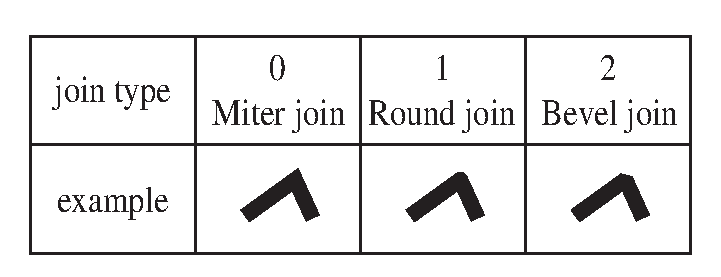
\includegraphics[width=9cm]{fig/join-type.pdf}\\

\vspace{5mm}
{\large \hspace{-1.5ex}$\bullet$ paint type:}\\
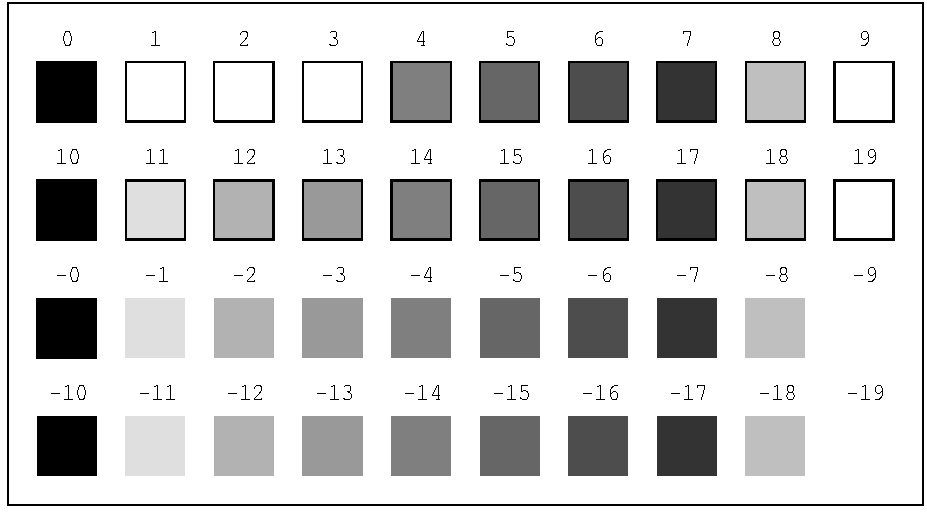
\includegraphics{fig/paint.pdf}\\
ps:~~~From $1 \sim 3$ only a frame is draw,
and for $-9$ and $-19$ the center is white and no frame is draw.

\end{qsection}
